\newpage
\subsection{Resultados}

\label{subsection:resultados}

	Esta subsección está dividida en cuatro partes. La primera etapa, está dedicada a replicar los resultados obtenidos por Wang et al. Estos valores van a conformar los baselines para los siguientes experimentos.

	La segunda, corresponde a los resultados obtenidos de haber entrenado y evaluado el clasificador Random Ferns con imágenes de caracteres en escenas naturales. Los gráficos mostrados en esta parte reflejan la relación entre la dimensión de los grupos y la precisión del clasificador.

	La tercera etapa contiene los resultados de haber reemplazado los caracteres reales del conjunto de entrenamiento por un conjunto de caracteres sintéticos (ver \ref{subsubsection:recon-caracteres}). El objetivo es demostrar cómo influye en la performance de clasificación el entrenar al clasificador con este tipo de imágenes. La relación que reflejan los gráficos es entre la precisión del clasificador y la cantidad de imágenes por conjunto de entrenamiento. Es decir, se van a evaluar diferentes conjuntos de entrenamiento, donde cada uno contiene una cierta cantidad de imágenes sintéticas.

	En la última parte, se procederán a mostrar los resultados de haber modificado el conjunto de entrenamiento de la segunda parte agregándole en diferentes proporciones imágenes sintéticas. Se compara este último enfoque con los anteriores para ver el impacto que produce en la performance dicho cambio.

	\subsubsection{Resultados de la implementación propia}
	\label{subsubsection: baseline-propio}

	Basados en el paper de Wang et al., se propuso realizar una reimplementación del trabajo realizado por los autores. Teniendo en cuenta los siguientes parámetros conocidos: cantidad de grupos = $256$ y bits por grupo = $6$ (con lo cual obtenemos vectores de características de longitud $1536$), se obtuvieron los resultados que se pueden apreciar en la tabla \ref{table: Baseline-Table}. En la misma, expresamos como ``NATIVE+FERNS'' a los resultados obtenidos al haber entrenado y evaluado el clasificador Random Ferns con imágenes reales. De la misma manera, ``SYNTH+FERNS'' se  refiere a los experimentos donde se usaron $1000$ imágenes sintéticas durante el entrenamiento.

	\begin{table}
		\centering
	    \begin{tabular}{ | l | l | l | p{5cm} |}
    			\hline
    				\textbf{Implementación} & \textbf{Score} \\ \hline
    				Wang NATIVE+FERNS & 54\% \\ \hline
    				Impl. propia NATIVE+FERNS & 50\% \\ \hline
    				Wang SYNTH+FERNS & 47\% \\ \hline
    				Impl. propia SYNTH+FERNS & 43\% \\

    			\hline
    		\end{tabular}
    		\caption[Resultados reales y sintéticas para baseline]{Resultados obtenidos en la reimplementación del trabajo de Wang et al.}
    		\label{table: Baseline-Table}
	\end{table}

	Como se puede ver en base a los resultados expuestos en el Cuadro \ref{table: Baseline-Table}, hay diferencias significativas entre los resultados de ambas implementaciones que se deben a varios factores. Existen ciertos parámetros que no están especificados en el trabajo de Wang et al. como es el caso del método de binarización utilizado. Basados en la implementación provista por los autores, se propuso, como método de binarización, la generación de variables aleatorias uniformes. Este enfoque resultó ser el más adecuado debido a que es el que más se asemeja a lo que hicieron los autores \cite{wang}. Otro parámetro no especificado fue el valor de \textit{alpha} para la inicialización de las tablas que influye en la performance. Asi mismo, la implementación de HOG que usan los autores es la desarrollada por Piotr Dollár \cite{PiotrD} la cual es una variación del método original propuesto por Dalal \& Triggs en \cite{DT05}. En la reimplementación se utiliza la función HOG extraida de la librería de python scikit-images, que también está basada en \cite{DT05} pero difiere de la usada por los autores. Una de las diferencias entre ambas funciones está en que la desarrollada por Piotr Dollar acepta imágenes a color y la que se usa en este trabajo sólo acepta imágenes en escala de grises. Otra diferencia entre estas implementaciones está en la longitud del vector resultante. Usando los mismos parámetros en ambas funciones, la desarrollada por Piotr Dollar devuelve vectores con una longitud $4$ veces mayor a los devueltos por la función HOG usada en el presente trabajo. Esto se debe a que usa un esquema deficiente de normalización.

	Ante esta situación se decide por establecer como baselines los resultados obtenidos por la configuración más cercana a la usada en \cite{wang}. Teniendo en cuenta los parámetros conocidos, se establecen además los siguientes: $8$ orientaciones y $9$ celdas por bloque para la función HOG; la generación de variables aleatorias uniformes entre dos puntos \textit{a} y \textit{b} como método para la binarización. Por último, el valor de \textit{alpha} se estableció en $0.01$ pues es el valor que más impacto positivo produjo en estos experimentos.

	En la siguiente sección, donde se van a mostrar los resultados de haber experimentado con imágenes reales, se va a tomar como baseline el valor $0.50$. De la misma manera, en los experimentos con imágenes sintéticas, el baseline pasará a ser $0.43$. Por último, en la sección sobre los experimentos con conjuntos de entrenamiento mixtos se van a mostrar ambos baselines.

	\subsubsection{Imágenes Reales}

	Los primeros 4 corresponden a los métodos utilizados en la binarización con lo cual se busca ver cual de los 4 arroja mejores resultados. Además, los primeros cuatro resultados reflejan la diferencia en performance al considerar grupos de diferente dimensión $\in \{ 1, 2, 4, 8, 10, 12\}$. Con esto buscamos establecer para cada caso, qué dimensión arroja los mejores resultados. Cabe aclarar que cada gráfico refleja la media de los resultados de 5 corridas del experimento junto con las barras de error a 1 desviación estándar. El quinto gráfico \ref{fig: Reales-Comparativa metodos} reune los mejores resultados de clasificación de los cuatro primeros, para establecer una comparación más precisa. La tabla \ref{table: reales-comparativa} se muestra un resumen de los mejores valores.

	 Dada la gran cantidad de parámetros que se manejan en estos experimentos, se va a dejar detallado en el análisis cuales son los mejores y se los va a usar para los siguientes experimentos.

			\begin{figure}[htbp!]
				\centering
				\centerline{
					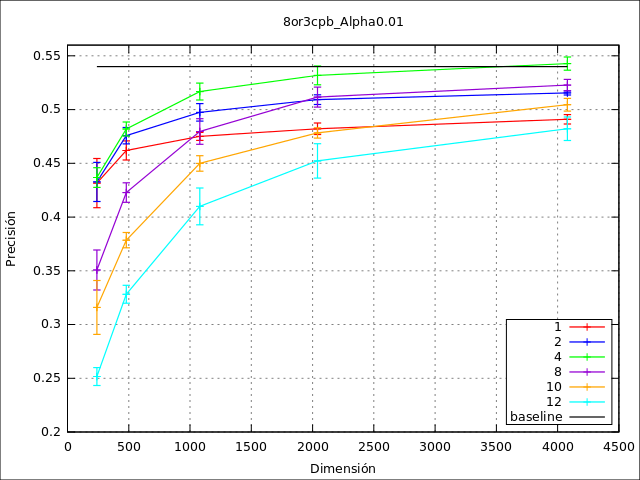
\includegraphics[scale=0.6]{img/resultados/reales/mean.png}
				}
				\caption[Resultados media]{Resultados usando la media}
				\label{fig: Reales-media}
			\end{figure}
			\begin{figure}[htbp!]
				\centering
				\centerline{
					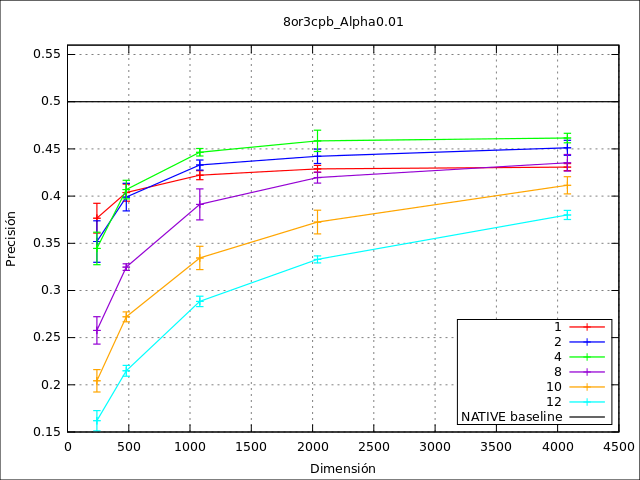
\includegraphics[scale=0.6]{img/resultados/reales/median.png}
				}
				\caption[Resultados mediana]{Resultados usando la mediana}
				\label{fig: Reales-mediana}
			\end{figure}
			\begin{figure}[htbp!]
				\centering
				\centerline{
					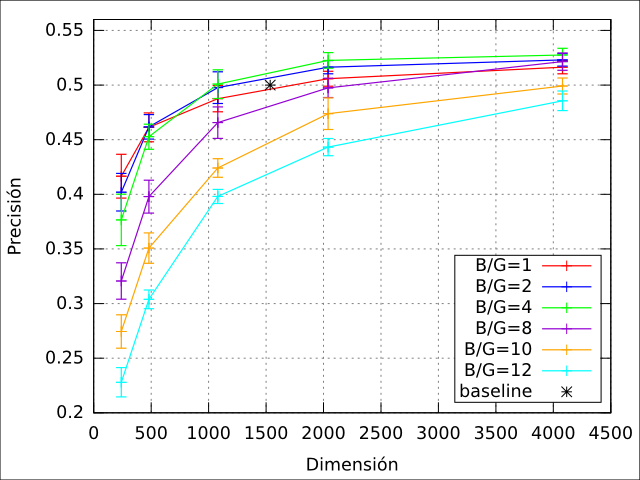
\includegraphics[scale=0.6]{img/resultados/reales/expon.png}
				}
				\caption[Resultados expon]{Resultados usando la distribución exponencial}
				\label{fig: Reales-expon}
			\end{figure}
			\begin{figure}[htbp!]
				\centering
				\centerline{
					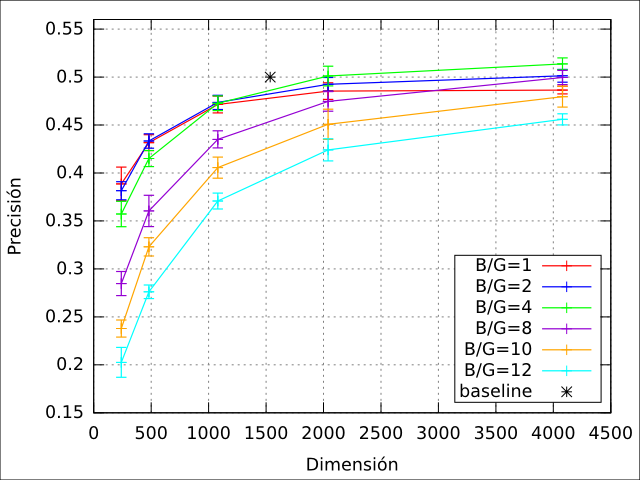
\includegraphics[scale=0.6]{img/resultados/reales/bootstrap.png}
				}
				\caption[Resultados bootstrap]{Resultados usando bootstrap}
				\label{fig: Reales-bootstrap}
			\end{figure}

	Teniendo en cuenta los resultados de los primeros $4$ gráficos, a simple vista se puede observar que los resultados obtenidos usando la media como método para binarizar los vectores son los mejores, llegando estos a un máximo cercano al $55\%$ de precisión. En el caso opuesto, el usar la mediana arrojó los peores resultados ya que en el mejor de los casos se supera el $47\%$ a diferencia de bootstrap que llega a $51\%$ . El uso de la distribución exponencial en los casos donde la longitud de los grupos es baja ($1$, $2$ bits por grupo) supera a la media en performance pero baja a medida que aumentamos este valor (casos $\{ 4, 8, 10, 12\}$ bits por grupo). Los valores que podemos encontrar en \ref{fig: Reales-expon} se acercan a los del a media llegando a un máximo en la precisión de $53\%$. En cuanto al uso de bootstrap, se puede apreciar que los resultados se mantienen por debajo de los obtenidos con la distribución exponencial y la media con valores que rondan entre $45\%$ y $52\%$.

	En cuanto a las dimensiones evaluadas $\{ 240, 480, 1080, 2040, 4080 \}$ es claro que a medida que aumentamos la longitud de los vectores aumenta la performance. Se puede ver que, cuando se usan vectores de longitud reducida (en este caso $240$), se marca una diferencia importante en la precisión entre los experimentos realizados con grupos de dimensionalidad baja $\{ 1, 2, 4 \}$ y alta $\{8, 10, 12\}$. Es decir, dejando fija la dimensión de los vectores en $240$, mientras más chico es el tamaño de los grupos mejor es el resultado (se puede observar en cualquiera de las figuras). En el otro extremo, si usamos grupos de $12$ bits la precisión disminuye considerablemente. La misma relación se mantiene a medida que aumentamos el tamaño de los vectores de características hasta cierto punto. Por ejemplo, en \ref{fig: Reales-media} es claro que a partir del uso de $1080$ como tamaño de vector en adelante, el uso de grupos de longitud mayor arroja mejores resultados. Lo mismo sucede en las otras figuras en diferentes puntos.

	En cuanto al uso del valor $4080$, se puede ver que no hay un aumento considerable en la performance que lo diferencie del uso de $2040$. Con esto en mente, es conveniente hacer uso de este último valor ya que usa vectores mucho más chicos incrementando la eficiencia en el cómputo.

	El problema con los vectores binarizados de dimensión reducida, es que almacenan menos correlaciones sobre los datos de la imagen a comparación de los vectores cuya longitud es mayor. Es decir, tal y como explicamos en \ref{subsection:ferns}, el vector se divide en grupos de dimensión \textit{S} con el objetivo de ir un paso más allá de la independencia propuesta en Na\"{i}ve Bayes donde cada dimensión es independiente. A nivel de grupo, se capturan las correlaciones entre las dimensiones involucradas, es decir, entre la información. Es por eso que al aumentar la dimensionalidad de los vectores en el proceso de binarización, capturamos más estructuras de correlación de los datos. Basándonos en esto, y como se puede observar en los gráficos expuestos, los grupos de $4$ bits son los más adecuados en la clasificación en la mayoría de los casos.

	Otro parámetro a analizar aquí es \textit{alpha} $\in \{ 0.0001, 0.001, 0.01, 0.1, 1\}$. Si recordamos la ecuación \ref{eq:Laplace-Smoothing}, en la cual hacemos uso del parámetro, podemos observar que el único objetivo de la misma es evitar que algunas de las entradas de la tabla del clasificador tengan el valor $0$ durante el entrenamiento. Si la cantidad de muestras es pequeña, como en nuestro caso, valores muy grandes de alpha van a generar que la ecuación retorne el mismo valor para la mayoría de los casos con lo cual tienden a sesgar la distribución a ser uniforme.  Esto genera que haya bastantes errores de clasificación. Los mejores resultados de cada método se dieron cuando el valor de \textit{alpha} se estableció en $0.01$ y son los que se muestran en la figura \ref{fig: Resultados-Reales}. Valores por encima $0.01$ o muy cercanos a 0 no llegaron en los experimentos a igualar la precisión obtenida con el valor de \textit{alpha} elegido. Por cuestiones de espacio se decidió mostrar en esta sección los resultados que se obtuvieron con el mejor valor. El resto de los gráficos se pueden encontrar en el apéndice ``B'' con el resto de los resultados de los experimentos.

	Al igual que con el parámetro \textit{alpha}, hay $2$ parámetros que se dejaron fijos y son los relacionados con la función de HOG: la cantidad de \textit{orientaciones} y la cantidad de \textit{celdas por bloque}. Se decidió por usar $8$ y $9$ respectivamente ya que dichos valores devuelven los mejores resultados.

			\begin{figure}[htbp]
				\centering
				\centerline{
					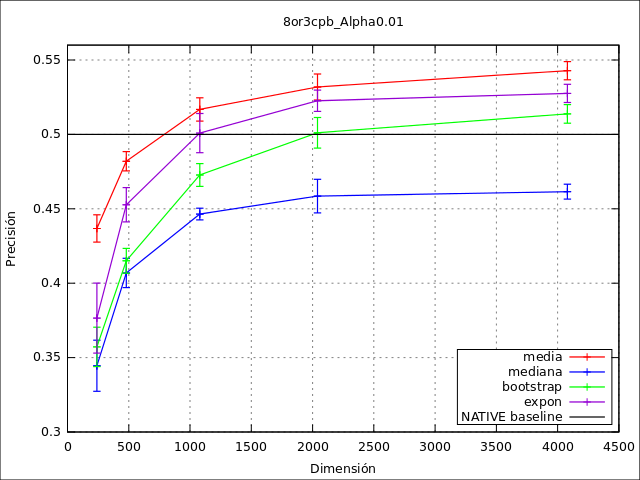
\includegraphics[scale=0.6]{img/resultados/reales/comparativa_metodos.png}
				}
				\caption[Reales comparativa]{El gráfico muestra las mejores curvas de los gráficos presentados con la mejor configuración}
				\label{fig: Reales-Comparativa metodos}
			\end{figure}

	Del análisis realizado surge que la mejor configuración está dada por \textit{alpha = $0.01$}, \textit{orientaciones = $8$}, \textit{celdas por bloque = $9$}, \textit{bits por grupo = $4$} y \textit{dimensión del vector = 2040}. Se puede observar en \ref{fig: Reales-Comparativa metodos} las mejores curvas para cada método utilizando la mejor configuración (a excepción de la longitud del vector con el objetivo de ver la curva de crecimiento). Queda claro que la media se puede establecer como el mejor método para la binarización por lo cual en los próximos experimentos se procederá a trabajar con el mismo. La diferencia en precisión entre usar vectores de longitud $2040$ y $4080$ no es notable en los $4$ casos por lo cual como dijimos anteriormente, el uso de $2040$ dimensiones permite obtener buenos resultados con un menor costo computacional. En todos los casos, salvo cuando se usa la mediana como método de binarización, se supera el baseline propuesto en diferentes puntos. La media logra una diferencia de $4\%$ con respecto al baseline pero usando vectores de dimensión $4080$, la misma diferencia baja a un $3\%$ si consideramos $2040$.

	La tabla \ref{table: reales-comparativa} muestra un resumen de los valores obtenidos con la mejor configuración para cada método.

	\begin{table}
		\centering
		\begin{tabular}{ | l | l | l | p{5cm} |}
    			\hline
    				\textbf{NATIVE + FERNS} & \textbf{Score} \\ \hline
    				Media & 53\% \\ \hline
    				Mediana & 46\%\\ \hline
    				Exponencial & 52\% \\ \hline
    				Bootstrap & 50\%\\
    			\hline
    		\end{tabular}
    		\caption[Resultados imagenes naturales]{Tabla comparativa entre los diferentes métodos propuestos para la binarización en la clasificación de caracteres en escenas naturales usando la mejor configuración de parámetros.}
    		\label{table: reales-comparativa}
    	\end{table}


    	\newpage
    	\subsubsection{Imágenes Sintéticas}

    En esta etapa se procederán mostrar los resultados obtenidos de los experimentos con las imágenes sintéticas. Además, los gráficos van a representar la relación entre la cantidad de imágenes sintéticas por clase (dado por \textit{IPC} en las siguientes figuras) y la precisión de clasificación dada por los $6$ valores a evaluar que son las dimensiones de los grupos. Teniendo en cuenta los resultados anteriores con las imágenes reales, se decidió por trabajar con la mejor configuración encontrada.

			\begin{figure}[htbp]
				\centering
				\centerline{
					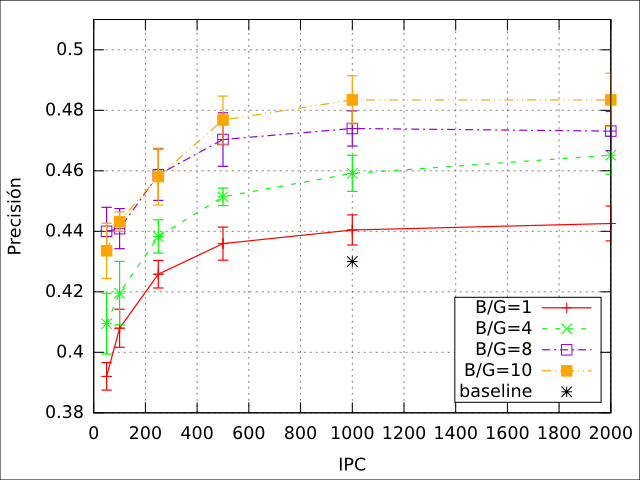
\includegraphics[scale=0.6]{img/resultados/sinteticas/mean_2040.png}
				}
				\caption[Sintéticas media 2040]{El gráfico muestra los resultados obtenidos de haber utilizado la mejor configuración analizada y haciendo uso de vectores binarizados de longitud $2040$}
				\label{fig: Sinteticas-media-2040}
			\end{figure}

	En cuanto a los experimentos con imágenes sintéticas, basándonos en los resultados plasmados en la figura \ref{fig: Sinteticas-media-2040}, es interesante observar que a medida que agregamos más imágenes sintéticas por clase sigue aumentando la performance del clasificador en todos los casos. Inicialmente, el crecimiento es más pronunciado hasta llegar a un punto (a partir de las 1000 IPC) en donde el mismo no es tan notable y en algunos casos tiende a ``aplanarse''. En base a esto, no tiene sentido trabajar con más de $1000$ imágenes por clase, pues computacionalmente es más costoso y no se obtiene una precisión que justifique su uso. En el mejor de los casos, al usar grupos de $12$ bits, la diferencia en performance entre usar $1000$ ó $2000$ imágenes por clase es de aproximadamente $0.0045$ o $1$ desviación standard. El hecho de que se hayan necesitado $2000$ muestras por clase para alcanzar una performance del $49\%$ también refleja que las imágenes sintéticas no aportan la misma cantidad de información que las reales.

	Por último, en cuanto a la comparación con el baseline obtenido en \ref{subsubsection: baseline-propio}, los resultados en la mayoría de los casos son superiores incluso habiendo entrenado al clasificador con menos imágenes por clase ($\leq 1000$).

\newpage
    	\subsubsection{Imágenes Reales y Sintéticas}

	Por último se van a mostrar los resultados correspondientes de haber entrenado al clasificador con conjuntos de entrenamiento mixtos. Se procederá a mostrar el gráfico con la mejor configuración. También se mostrarán las matrices de confusión para este caso. Teniendo en cuenta el análsis anterior, se van a mostrar el resultado de haber utilizado solamente la media como umbral ya que fue la que retornó los mejores valores.

	El gráfico a continuación presenta el eje \textit{x} en escala logarítmica para poder apreciar mejor las variaciones que se dan al experimentar con valores cercanos entre sí.

			\begin{figure}[!htbp]
				\centering
				\centerline{
					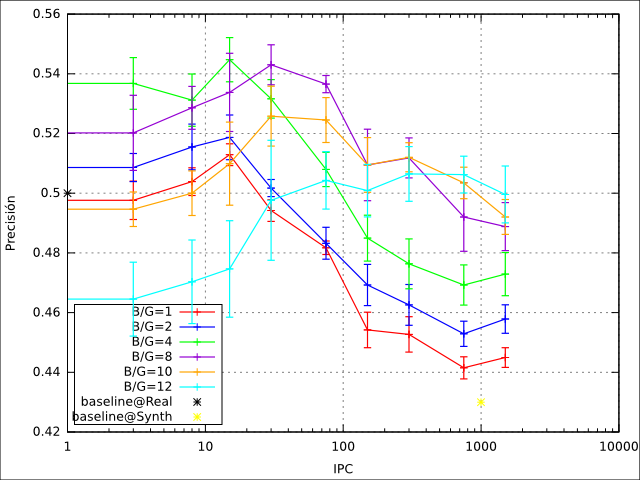
\includegraphics[scale=0.6]{img/resultados/mixtas/best_mean_2040.png}
				}
				\caption[Mixtas media mejor resultado]{El gráfico muestra la configuración que devolvió los mejores resultados.}
				\label{fig: Mixtas-media-mejor}
			\end{figure}

	De la figura \ref{fig: Mixtas-media-mejor} se puede desprender el siguiente análisis. El primero, y uno de los más importantes, hace referencia a la influencia en la clasificación de ir agregando de manera incremental imágenes sintéticas durante la etapa de entrenamiento. Se puede observar que a nivel general todos los experimentos llegaron a un punto donde su performance se desplomó al seguir agregando imágenes. Sin embargo, este cambio ocurrio en diferentes momentos dependiendo del caso. Por ejemplo, cuando trabajamos con grupos de dimensionalidad baja ($1$, $2$ y $4$ bits por grupo), la precisión del clasificador va en aumento hasta que se llega a un máximo correspondiente al haber entrenado al sistema con igual cantidad de imagenes reales y sintéticas. A partir de ese punto el seguir incrementando la proporción de sintéticas sobre reales trajo efectos negativos en los resultados como se puede apreciar en el gráfico presentado. En los casos donde consideramos $10$ bits por grupo el rendimiento se desploma cuando consideramos más de 75 imágenes sintéticas. La curva presentada por el grupo de $12$ bits es llamativa ya que a diferencia del resto, sigue incrementando su performance hasta que llega al punto máximo cuando consideramos entrenar al clasificador con $50$ veces más imágenes sintéticas que reales. Cuando superamos esa proporción se puede ver que la performance decae.

	 La mejor curva en el gráfico la obtenemos cuando consideramos $4$ bits por grupo y entrenamos al clasificador con la misma cantidad de imágenes sintéticas que reales. Este resultado coincide respecto al análisis realizado para los experimentos con imágenes reales donde consideramos que el mejor parámetro era considerar grupos de $4$ bits. En la mayoría de los casos se dan buenos resultados cuando la cantidad de imágenes sintéticas sobre las reales es la misma ($1$, $2$ y $4$) o se duplica ($8$ y $10$).

	 Teniendo en cuenta los baselines presentados en la tabla \ref{table: Baseline-Table}, no queda la menor duda que por el simple hecho de tener una base de imágenes reales el baseline ``SYNTH'' se ve ampliamente superado. En cuanto al baseline ``NATIVE'', a diferencia de los resultados obtenidos con las imágenes reales (que se pueden ver en el inicio de cada curva de la figura \ref{fig: Mixtas-media-mejor}), el incremento en la precisión del clasificador no es muy notorio; sin embargo, el hecho de poder incrementar la performance haciendo uso de imágenes sintéticas es un avance. Llama la atención que el usar la misma cantidad de imágenes reales y sintéticas no haya producido un incremento más marcado en la performance. Sin embargo, como pudimos ver en \ref{fig: Sinteticas-media-2040}, ni con 50 imágenes sintéticas por clase se podía alcanzar un valor similar al del baseline.

	Uno de los análisis más interesantes del trabajo, pasa por los errores de clasificacion que se han observado. En las figuras \ref{fig: Mixtas-Matrix-media-mejor} y \ref{fig: MatrizIns-Mixtas-media-mejor}, se pueden ver dos matrices de confusión. La primer corresponde al mejor resultado obtenido en la figura \ref{fig: Mixtas-media-mejor} y la segunda es una versión de la primera donde no diferenciamos caracteres mayúsculas de minúsculas.

	En la región central, dada por la diagonal de la matriz, se encuentran las muestras que fueron bien clasificadas durante la evaluación del clasificador. Existen zonas dentro de la diagonal que corresponden a clases que obtuvieron una tasa de acierto inferior al $30\%$ (los cuadrados en escala de azul dentro de la imagen). En estas clases son más comunes los siguientes errores:

	\begin{itemize}
		\item No poder distinguir mayúsculas de minúsculas para los caracteres involucrados. En la figura \ref{fig: Error-CaseSensitive} se puede observar un ejemplo donde, incluso para las personas, es difícil notar la diferencia.
		\item Confundir un carácter por otro similar. La figura \ref{fig: Error-Apariencia} muestra varios ejemplos donde se pueden confundir caracteres.
	\end{itemize}

		\begin{figure}[htbp]
			\centering
			\subfloat[c minúscula\label{fig: Lower-case-c}]{
				\fbox{ 
\includegraphics[scale=1]{img/errores_clasif/CaseSensitiveError/lowerCase_c.png} }
			}
			\subfloat[C mayúscula\label{fig: Upper-case-C}]{
				\fbox{ 
\includegraphics[scale=1]{img/errores_clasif/CaseSensitiveError/upperCase_C.png} }
			}
			\subfloat[z minúscula\label{fig: Lower-case-z}]{
				\fbox{
\includegraphics[scale=1]{img/errores_clasif/CaseSensitiveError/lowerCase_z.png} }
			}
			\subfloat[Z mayúscula\label{fig: Upper-case-Z}]{
				\fbox{ 
\includegraphics[scale=1]{img/errores_clasif/CaseSensitiveError/upperCase_Z.png} }
			}
			\\
			\subfloat[x minúscula\label{fig: Lower-case-x}]{
				\fbox{ 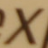
\includegraphics[scale=1]{img/errores_clasif/CaseSensitiveError/lowerCase_x.png} }
			}
			\subfloat[X mayúscula\label{fig: Upper-case-X}]{
				\fbox{ 
\includegraphics[scale=1]{img/errores_clasif/CaseSensitiveError/upperCase_X.png} }
			}
			\subfloat[v minúscula\label{fig: Lower-case-v}]{
				\fbox{ 
\includegraphics[scale=1]{img/errores_clasif/CaseSensitiveError/lowerCase_v.png} }
			}
			\subfloat[V mayúscula\label{fig: Upper-case-V}]{
				\fbox{ 
\includegraphics[scale=1]{img/errores_clasif/CaseSensitiveError/upperCase_V.png} }
			}
			\caption[Error entre mayúscula y minúscula]{Error de clasificación donde se confunde el caracter en mayúscula y en minúscula.}
			\label{fig: Error-CaseSensitive}
		\end{figure}

		\begin{figure}[htbp]
			\centering
			\subfloat[o minúscula\label{fig: Lower-case-o}]{
				\fbox{ 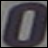
\includegraphics[scale=1]{img/errores_clasif/ShapeError/lowerCase_o.png} }
			}
			\subfloat[O mayúscula\label{fig: Upper-case-O}]{
				\fbox{ 
\includegraphics[scale=1]{img/errores_clasif/ShapeError/upperCase_O.png} }
			}
			\subfloat[número 0\label{fig: Number-0}]{
				\fbox{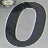
\includegraphics[scale=1]{img/errores_clasif/ShapeError/number_0.png} }
			}
			\\
			\subfloat[I mayúscula\label{fig: Upper-case-I}]{
				\fbox{ 
\includegraphics[scale=1]{img/errores_clasif/ShapeError/upperCase_I.png} }
			}
			\subfloat[l minúscula\label{fig: Lower-case-l}]{
				\fbox{ 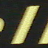
\includegraphics[scale=1]{img/errores_clasif/ShapeError/lowerCase_l.png} }
			}
			\subfloat[número 1\label{fig: Number-1}]{
				\fbox{ 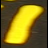
\includegraphics[scale=1]{img/errores_clasif/ShapeError/number_1.png} }
			}
			\caption[Error de apariencia]{Error de apariencia entre caracteres.}
			\label{fig: Error-Apariencia}
		\end{figure}


	El no poder distinguir mayúsculas de minúsculas se ve reflejado en la matriz \ref{fig: MatrizIns-Mixtas-media-mejor} en dos regiones. Dichas regiones corresponden a dos submatrices, la primera ubicada en la esquina inferior izquiera y la segunda en la esquina superior derecha. Ambas submatrices, no involucran los caracteres numéricos y se puede ver en la diagonal de cada una, la cantidad de imágenes de cada clase donde se confundió la versión mayúscula y minúscula. Es muy difícil, incluso para las personas, clasificar imágenes de caracteres recortados donde no hay una clara distinción entre la versión mayúscula y minúscula.

	Los errores de ``apariencia'' como los expuesto en la figura \ref{fig: Error-Apariencia} estan distribuidos por toda la matriz, habiendo casos donde la similitud es evidente y en otros casos más raros donde no existe directamente. Este último caso, donde no existe similitud, puede solventarse si se entrenase al clasificador con más imágenes.

	La matriz \ref{fig: MatrizIns-Mixtas-media-mejor} se creó con el objetivo de reflejar otra punto de vista de los resultados, donde no se consideren los caracteres en mayúscula. Se puede observar que la diagonal de la matriz mejora con respecto a la anterior y además se acentúan aún más los problemas de apariencia que surgen entre ciertos caracteres. Por ejemplo, los errores de clasificación en el carácter ``i'' que se confunde con una ``l'' en muchos casos o el carácter ``o'' con el número ``0''. La mayoría de los errores de clasificación se podrían corregir si se tuviera un mejor método para generar caracteres sintéticos ya que, como se pudo observar en los resultados, los usados en este trabajo no pudieron superar en precisión al conjunto de imágenes reales.



			\begin{figure}[!htbp]
				\centerline{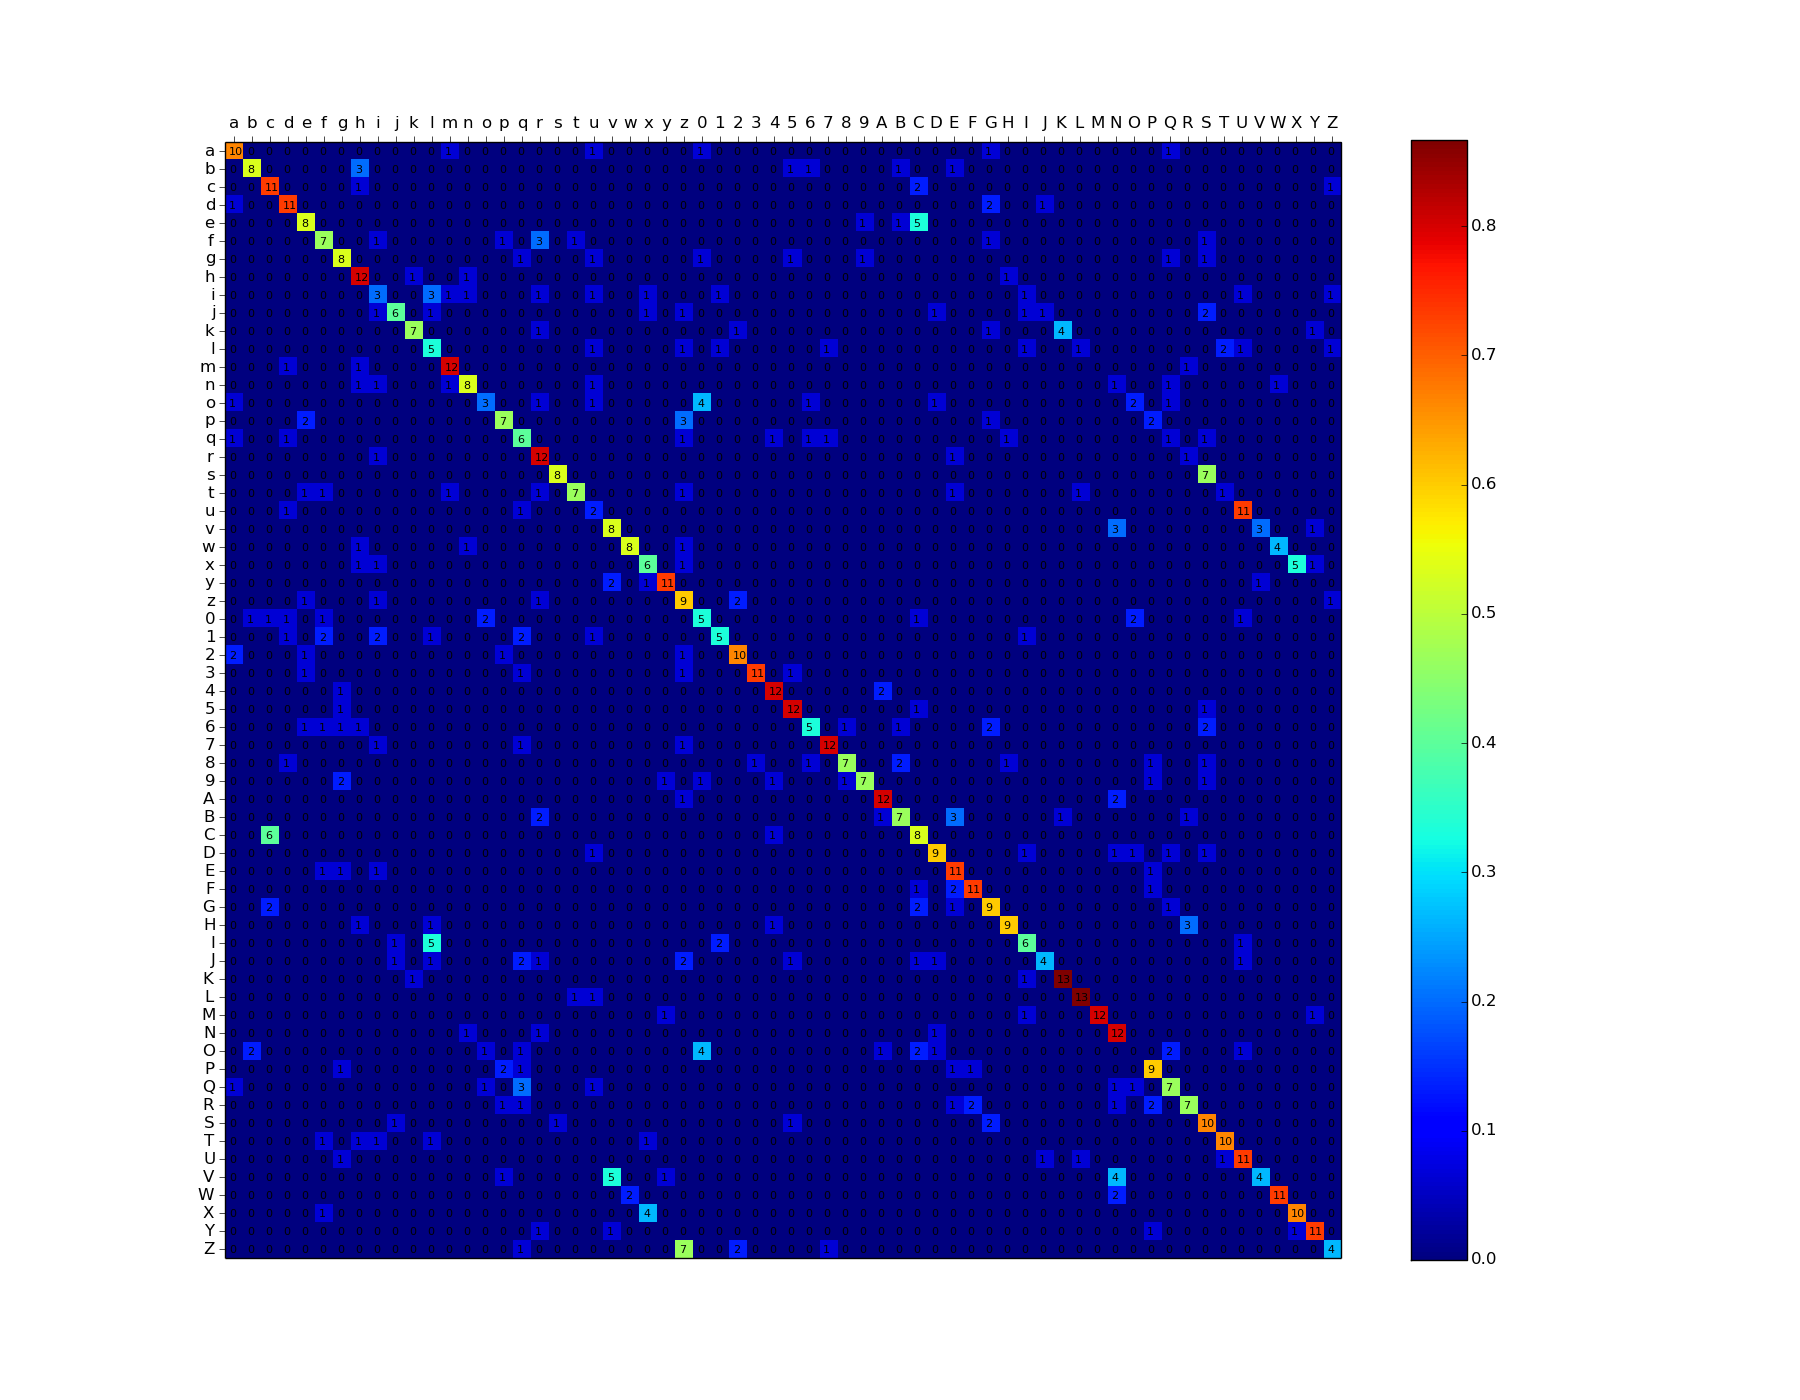
\includegraphics[scale=0.4]{img/resultados/mixtas/best_mean_matrix_Alpha0,01_2040-4.png}}
				\caption[Mixtas Matriz expon]{Matriz de correlación del gráfico \ref{fig: Mixtas-media-mejor} para el mejor resultado. \RC{Demasiado grande las matrices como para mostrarlas y que se vean bien}}
				\label{fig: Mixtas-Matrix-media-mejor}
			\end{figure}

			\begin{figure}[!htbp]
				\centerline{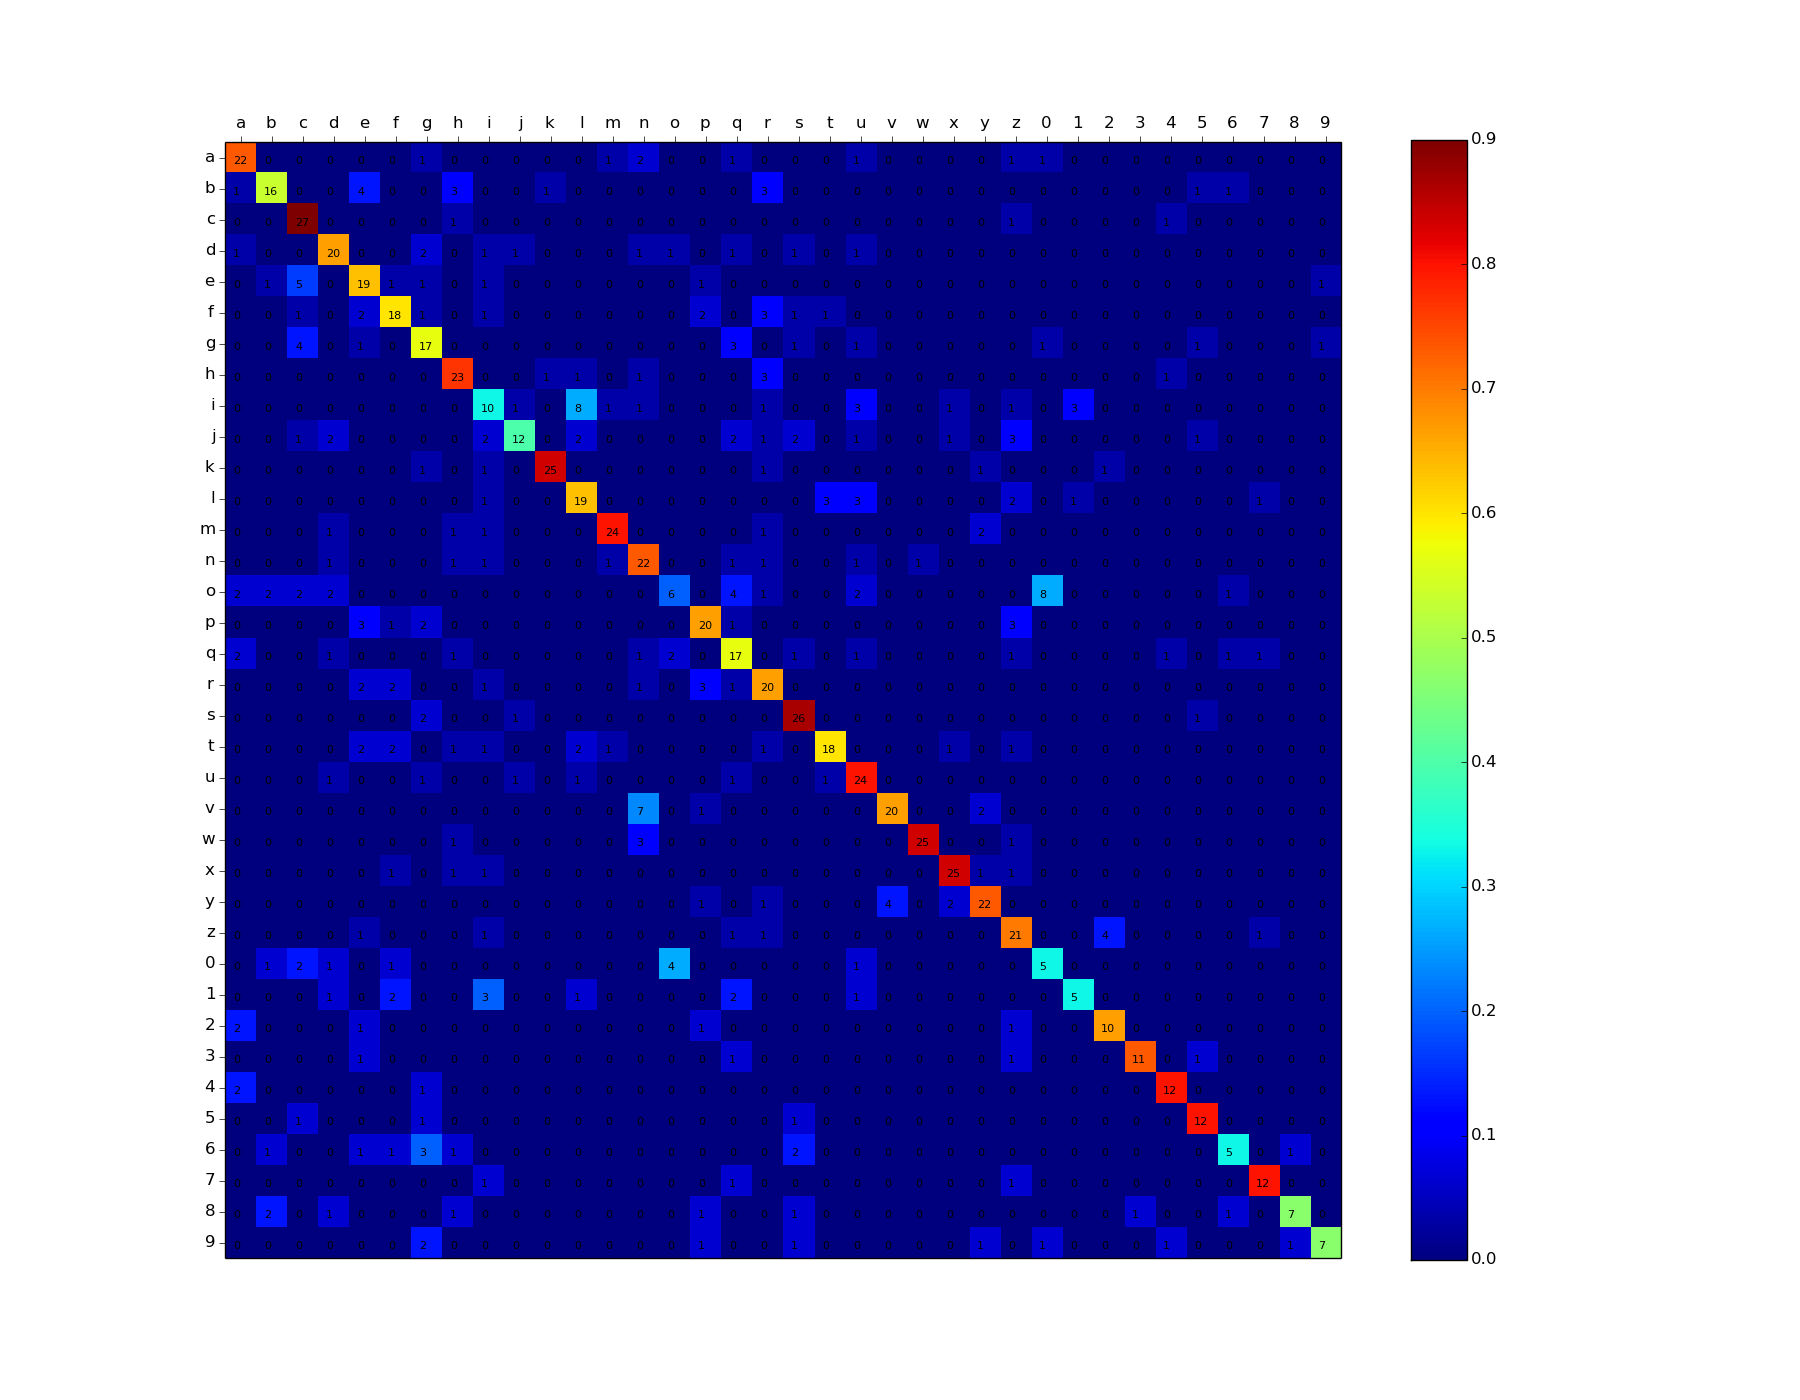
\includegraphics[scale=0.4]{img/resultados/mixtas/best_mean_matrix_Alpha0,01_2040-4_ins.png}}
				\caption[Matriz de correlación ``case insensitive'' para mixtas media]{Matriz de correlación del gráfico \ref{fig: Mixtas-media-mejor} para el mejor resultado no teniendo en cuenta los caracteres en mayúscula.}
				\label{fig: MatrizIns-Mixtas-media-mejor}
			\end{figure}
